\documentclass[12pt]{article}

\setlength{\parskip}{1ex}
\addtolength{\textwidth}{.8in}
\addtolength{\textheight}{.2in}
\setlength{\oddsidemargin}{.2in}
%\usepackage{showkeys}

\usepackage{graphicx,amsmath,amssymb,wrapfig,color,amsfonts}
\usepackage[section]{placeins}
%\usepackage{showkeys}
\usepackage{enumitem}

\newcommand{\SWE}{shallow water equations }
\newcommand{\onehalf}{\frac{1}{2}}
%\newcommand{\pr}[1]{\frac{\partial #1}{\partial m}}
\newcommand{\pr}[1]{{#1}_m}
\newcommand{\rhot}{\widetilde{\rho}}
\newcommand{\rhoh}{\widehat{\rho}}
\newcommand{\ut}{\widetilde{u}}
\newcommand{\uh}{\widehat{u}}
\newcommand{\wt}{\widetilde{w}}
\newcommand{\wh}{\widehat{w}}
\newcommand{\pt}{\widetilde{p}}
\newcommand{\ph}{\widehat{p}}
\newcommand{\htil}{\widetilde{h}}
\newcommand{\hh}{\widehat{h}}
\newcommand{\commentout}[1]{}

\begin{document}

\title{A State Redistribution Algorithm for Cut Cells}
\author{Marsha Berger\footnote{Courant Institute, New York University, 251 Mercer St.,
NY, NY 10012}  \hspace{1in} Andrew Giuliani $^*$}

\maketitle

\begin{abstract}
\end{abstract}

\section{Introduction}\label{sec:intro}
Cut cell meshes to solve hyperbolic problems 
are increasingly prevalent due to the ease 
of grid generation for complicated geometries \cite{}. 
However the {\em small cell} problem is still an active area of research, and
a completely satisfactory solution has not yet been found.
The small cell problem can be explained as follows: explicit
finite volume schemes typically need to take a time step 
that is proportional to the mesh width in order to satisfy a CFL constraint for
stability. However cut cells can have volumes that are arbitrarily
smaller than the regular cells that would otherwise determine the stable time
step. Special algorthms are needed to prevent this restriction.

The most commonly used stabilization algorithm is called flux
redistribution \cite{chern:colella,vof:colella}. The main idea is illustrated below in two space
dimensions, for ease of notation.
The essential idea is to compute the 
flux update for a cut cell $i,j$ with volume $V_{i,j} < V_{\mbox{\em full}}$,
\begin{eqnarray*}
V_{i,j} Q_{i,j} ^{n+1} & = V_{i,j} Q_{i,j}^n  +  \Delta t \, \Sigma_k F_k \cdot l_{k}\\
                   & = V_{i,j} Q_{i,j}^n  +  \delta  M 
\end{eqnarray*}
Here, $V_{\mbox{\em full}}$ is the volume of a full uncut cell.
Instead of using the entire amount of the update in cell ${i,j}$, 
the cut cell only uses a fraction $\eta$ of it.  If the fraction $\eta$
is proportional to the cell's volume
fraction $V_{i,j}/V_{\mbox{\em full}}$, the update should be stable. 
To maintain conservation, the rest of the update ($1-\eta)\delta M$
is given to the cell's neighbors.  
There are more recent additional steps that make the distribution 
more robust and accurate. For example, the difference between a stable
non-conservative update and the conservative update is what is
redistributed (see \cite{} for details).
Flux redistribution has already been implemented for three dimensional
calculations due to its simplicity. However it is only first order
accurate at the cut cells.

Cell merging is most frequently the first idea people 
think of. It is conceptually simple, but 
we are not aware of any production codes that implement this in a fully
general, robust manner for complicated engineering geometries. 
The $h$-box method \cite{mjb-hel-rjl:hbox2,mjb-hel:hboxsimple}
is a second order accurate method at the cut cells. It extends the 
domain of dependence for the fluxes around a small cell in a 
special way that maintains stability by means of a cancellation
property. It  has not been extended to
three dimensions due to its complexity. 

In Schneiders et al \cite{shws:2011}, the authors make
some improvements to flux redistribution for viscous flow in moving
geometries. They introduce a
smooth cutoff function of cell size for when it is applied. They also
use a non-uniform weighting in the gradient stencil to avoid abrupt
changes, which can lead to oscillations in the solution. This is
especially important for moving geometries.

In \cite{BalajiMenon:2016}, the authors also tackle viscous flow, with a
third order accurate (or higher) approach. They use a cluster of cells,
akin to cell merging, but maintain each cell's identity. A high order
polynomial is fit to the cluster, and replaces the solution values in the
individual cells.  Our algorithm has a similar spirit to this, though the
details are very different. HARD TO UNDERSTAND WHAT THE DO

In \cite{May-Berger:JSC}, an implicit scheme was developed to
handle stability of the cut cells, and was combined with an 
explicit method for the full cells. In this work we will focus on 
two explicit methods, and make modification necessary for them accuracy 
on the cut cells.
Other approaches that have been proposed in the literature include
interpolation-based procedures, such as the mirror-cell method by Forrer
and Jeltsch \cite{article:FoJe98}, and a related ghost-fluid method by
Dadone and Grossman \cite{DadoneGrossman}.
There are also approaches based on finite difference schemes
\cite{SjogreenPetersson,MarcoBjorn}
and kinetic schemes \cite{Oksuzoglu:thesis,KeenKarni}.
However, since we are interested in methods
that preserve conservation we do not explore these alternatives further.

In this paper we propose a framework for a stabilization algorithm in
the spirit of flux redistribution (henceforth FRD). 
As with FRD, it is applied as a postprocessing
step, and is simple to implement. Cell updates on all cells are performed
in the usual way, followed by a postprocessing step based on the
conserved state variables, not on the fluxes.
Hence we call it {\em state redistribution} (SRD).


To set the stage, notice that cell merging itself can
be rewritten as a postprocessing step.
\commentout{
To take one step to update a finite volume approximation to
$u_t + u_x = 0$ we do the following:
\begin{itemize}
\setlength\itemsep{.2in}
\item
{\bf Finite Volume Step}\\
Take the usual finite volume step with fixed, regular  $\Delta t$ on all cells 
including the small cell:
\begin{equation}
\bar{u}_j = u_j^n - \frac{\Delta t}{h_j} \; (f_{j+1/2} - f_{j-1/2} ), 
\quad \forall j.
\label{eqn:fvupdate}
\end{equation}

\item
{\bf {\em Temporarily} Create Merged Cell}\\
Temporarily create the {\em merged} cell $\overline{u_M}$ consisting of the small cell $u_j$ and one
or both of its neighbors so that it the merged cell is of sufficient
size (to be discussed later).  For simplicity here we will merge 
only with the neighbor on the right,
\begin{equation}
\widehat{q_M} =  \frac{ h_k \bar{u}_k + h_{k+1} \bar{u}_{k+1} } {h_k +
h_{k+1}} .
\label{eqn:mergestep}
\end{equation}

\item
{\bf Compute Merge Cell Gradient }\\
There are several ways to do this. 
Two simple possibilities are 
\begin{equation}
\nabla \widehat{u_M} = \frac{\bar{u}_{k+2} - \bar{u}_{k-1}} {x_{k+2}-x_{k-1}}
\label{eqn:gradLim1}
\end{equation}
which does not use the merged cell,
or
\begin{equation}
\nabla \widehat{u_M} = \frac{\bar{q}_{k+2} - \widehat{u_{M}}} {x_{k+2}-x_{M}}
\label{eqn:gradLim2}
\end{equation}
which uses the merged cell, and $x_M$ is the centroid of the merged
cell.
The choice of gradient stencil will be studied later in section \ref{sec:srdAlg}.

%Other more accurate alternatives exist, not all of which are stable.
%It would be better to use smaller stencils, perhaps including $u_{k+1}$
%or $\overline{u_M}$ itself.

\item
{\bf Redistribute Merged State to Cells Comprising Merged cell }\\
Replace the provisional values computed in the cells comprising the
merged cell with the merged solution reconstructed to the cell
centroids:
\begin{equation}
\begin{split}
u_k^{n+1} &= \widehat{u_M} +  (x_k - x_M) \nabla \widehat{u_M}\\
u_{k+1}^{n+1} &= \widehat{u_M} +  (x_{k+1} - x_M) \nabla \widehat{u_M}
\end{split}
\end{equation}
\end{itemize}
}
First  update cells $k$ and $k+1$, shown in Figure \ref{fig:modelProblem1},  using a standard finite volume scheme
with fixed $\Delta t$ on all cells:
\begin{equation}
\bar{u}_j = u_j^n - \frac{\Delta t}{h_j} \; (f_{j+1/2} - f_{j-1/2} ), 
\quad \forall j.
\label{eqn:fvupdate}
\end{equation}
Next form the merged cell
\begin{equation}
\widehat{q_M} =  \frac{ h_k \bar{u}_k + h_{k+1} \bar{u}_{k+1} } {h_k +
h_{k+1}} .
\label{eqn:mergestep}
\end{equation}
which works out to
\begin{equation}
\widehat{q_M} = \widehat{q_M}^n - 
\frac{\Delta t}{h_k + h_{k+1}} (f_{k+3/2} - f_{k-1/2})
\end{equation}

\begin{figure}
\begin{center}
%\vspace*{-.5in}
\includegraphics[height=1.3in]{figs/1dfig.pdf}
\caption{\sf Notation for model problem in one space dimension. The small
cell has size $\alpha h$ in a mesh with regular mesh width $h$.}
\label{fig:modelProblem1}
\end{center}
\end{figure}


For the simplest first order version, we simply set
\begin{equation}
u_k^{n+1} = u_{k+1}^{n+1} = \widehat{q_M}^{n+1} 
\label{eqn:finalstep}
\end{equation}
Recognizing that $h_k+h_{k+1}$ is the merged cell volume makes 
clear the relationship to cell merging.
If the final update step \eqref{eqn:finalstep}  is replaced by 
\begin{equation}
\begin{split}
u_k^{n+1} &= \widehat{q_M} +  (x_k - \widehat{x}_M) \,\, \nabla \widehat{q_M}\\
u_{k+1}^{n+1} &= \widehat{q_M} +  (x_{k+1} - \widehat{x}_M) \, \nabla \widehat{q_M}
\end{split}
\end{equation}
then the method is linearity preserving, 
if all gradients are computed accurately enough to preserve a linear function.  

By using a higher than linear polynomial and
including more neighbors in the
redistribution (on top of a more accurate finite volume scheme for the
entire mes ),
we have a path to higher order accuracy.
The method is also conservative since the mass of the merged cell equals the 
mass of the two cells comprising it.



The choice of merging neighborhoods and gradients is what makes up the
specifics of SRD in two space dimensions. Furthermore, it can happen
that a cell has more than one neighborhood with
which it should merge. This is what often causes complications in cell
merging algorithms. In SRD, we will simply use all such values appropriately
weighted.

In the next section  we first review the finite volume schemes to which SRD will
be applied.
The SRD algorithm in two space dimensions will be presented in section
\ref{sec:srdAlg}.
For simplicity we present the second order accurate version first.
The more general higher order extension is described in 
section \ref{sec:ho}.
Some theoretical results using one-dimensional model problems are in
section \ref{sec:theory}. 
Section \ref{sec:compResults} shows computational results for both smooth
problems and shocked flow for both linear advection and the Euler equations.  We conclude in section \ref{sec:conc}.



\section{Finite volume method}
We use the finite volume spatial discretization 
\begin{equation} \label{eq:fv}
\frac{d}{dt}(U_{i,j}) =  - \frac{1}{h_i} \int_{\partial \Omega_{i,j}} \mathbf{F}^* \cdot \mathbf{n}~dl,
\end{equation}
where $\mathbf{n}$ is the outward facing normal, $\mathbf{F} = \mathbf{F}^*(u_l,u_r)$ and $u_{i,j}(x,y)$ is a polynomial reconstruction of the solution on cell $i$ of the form
\begin{equation}\label{eq:u}
\begin{aligned}
	    u_{i,j}(x,y) = U^n_{i} +  \sigma_{i,j,x}\frac{x- x_{i,j}}{\Delta x} +   \sigma_{i,j,y}\frac{y- y_{i,j}}{\Delta y} + \frac{1}{2} \delta_{i,j, xx}\left[ \frac{(x -  x_{i,j})^2 }{\Delta x^2} -  M_{i,xx}\right]\\
	    + \delta_{i,j, xy}\left[ \frac{(x -  x_{i,j}) (y -  y_{i,j}) }{\Delta x \Delta y} -  M_{i,xy}\right] + \frac{1}{2} \delta_{i,j, yy}\left[ \frac{(y -  y_{i,j})^2 }{\Delta y^2} -   M_{i,yy}\right]\\
	     + \frac{1}{6}\gamma_{i,j, xxx}\left[ \frac{(x -  x_{i,j})^3 }{\Delta x^3} -  M_{i,xxx}\right] + \frac{1}{2}\gamma_{i,j, xxy}\left[ \frac{(x -  x_{i,j})^2 (y -  y_{i,j}) }{\Delta x^2 \Delta y} -  M_{i,xxy}\right]\\
	     + \frac{1}{2}\gamma_{i,j, xyy}\left[ \frac{(x -  x_{i,j}) (y -  y_{i,j})^2 }{\Delta x \Delta y ^2} -  M_{i,xyy}\right]+ \frac{1}{6}\gamma_{i,j, yyy}\left[ \frac{(y -  y_{i,j})^3 }{\Delta y^3} -  M_{i,yyy}\right],
\end{aligned}
\end{equation}
and $ x_{i,j}$, $ y_{i,j}$ is the centroid of cell $i$. $\sigma_{i,j,x}$, $ \sigma_{i,j,y}$, $ \delta_{i,j,xx}$, $ \delta_{i,j,xy}$, $ \delta_{i,j,yy}$, $ \gamma_{i,j,xxx}$, $ \gamma_{i,j,xxy}$, $ \gamma_{i,j,xyy}$, $ \gamma_{i,j,yyy}$, are the first, second, and third derivatives, and $  M_{i,xx}$, $ M_{i,xy}$,  $ M_{i,yy}$ are geometric constants. We find the derivatives of the polynomial reconstruction that satisfy the following in a least squares sense
\begin{equation}\label{eq:qi}
\frac{1}{ V_j}\int_{\Omega_j} u_i(x)~d\Omega_j = U_j \quad \forall j \in R_i,
\end{equation}
where $R_i$ is the set of indices of neighborhoods used for reconstruction on merging neighborhood $i$.  For the Euler equations, this reconstruction is done in primitive rather than conserved variables.  The surface integral in \eqref{eq:fv} is evaluated using a Gaussian quadrature rule of degree $p$, where $p$ is the degree of the polynomial reconstruction.  \eqref{eq:fv} is advanced in time using a Runge-Kutta scheme of order $p+1$.



\subsection{High-order limiting on non-coordinate aligned meshes}
\subsubsection*{Full cells}
Consider now the case when $p=1$
\begin{align*}
\tilde \sigma_{x,i,j} &= \text{minmod}(2( U^n_{i+1,j}- U^n_{i,j}), \sigma_{x,i,j}, 2( U^n_{i,j}- U^n_{i-1,j}))\\
\tilde \sigma_{y,i,j} &= \text{minmod}(2( U^n_{i,j+1}- U^n_{i,j}), \sigma_{y,i,j}, 2( U^n_{i,j}- U^n_{i,j-1})).
\end{align*}
Consider now the case when $p=2$
\begin{align*}
\tilde \delta_{i,j,xx} &= \text{minmod}(2( \sigma_{i+1,j,x}- \sigma_{i,j,x}), \delta_{i,j,xx}, 2( \sigma_{i,j,x}- \sigma_{i-1,j,x}))\\
\tilde \delta_{i,j,xy} &= \text{minmod}(2( \sigma_{i,j+1,x}- \sigma_{i,j,x}),2( \sigma_{i+1,j,y}- \sigma_{i,j,y}), \delta_{i,j,xy}, 2( \sigma_{i,j,x}- \sigma_{i,j-1,x}),2( \sigma_{i,j,y}- \sigma_{i-1,j,y}))\\
\tilde \delta_{i,j,yy} &= \text{minmod}(2( \sigma_{i,j+1,y}- \sigma_{i,j,y}), \delta_{i,j,yy}, 2( \sigma_{i,j,y}- \sigma_{i,j-1,y}))
\end{align*}

\subsubsection*{Cut cells}


\section{The State Redistribution Algorithm}\label{sec:srdAlg}

In this section we describe only the second order accurate version of the State
Redistribution Algorithm. 
This helps simplify the notation and make the
algorithm more intuitive.   
At several places there are choices
to make, and we discuss the alternatives and the reason behind our
choices.  Since the postprocessing step comes after the finite
volume update step, we begin this section by briefly reviewing the 
two methods that SRD is applied to.  

\subsection{The Base  Finite Volume Schemes}

Our computational results will use two different finite volume schemes
to update the Cartesian cut cell mesh.
We will refer to these at the base schemes. 
The  update is applied to the entire mesh, including  
to the small cut cells.  Since cut cells can have cell volumes that are
orders of magnitude smaller than the time step allowed by the full
cells, these will lead to instability without a stabilization algorithm.
SRD will be applied after each stage or step of the base scheme.

\begin{figure}
\begin{center}
\includegraphics[width=2.8in]{figs/2dfig.pdf}
\caption{\sf Notation for mesh in two space dimensions. The cells shaded
in yellow are the cut cells.} 
\label{fig:2dfig}
\end{center}
\end{figure}

\subsubsection{Method of Lines approach}
The simplest scheme is to use a spatial discretization over the entire
mesh, and apply a Runge-Kutta scheme in time. This is a well-known
standard approach
on regular Cartesian meshes. It is adapted for the cut cells by
using a least squares reconstruction of the gradient that includes
either edge and node neighbors (unless otherwise specified).
Limiting is done using the Barth-Jespersen limiter \cite{} 
on the cut cells and one adjacent neighbors. Any limiter
can be used for the regular cells.

The spatial reconstruction in the cut cells is no longer
coordinate-aligned, and is modified
to include both $x$ and $y$ components of the gradient to 
reconstruct to the midpoint of the cell edge. This is indicated 
in figure \ref{fig:2dfig}  with a green $\times$.
The SRD stabilization scheme is applied after each stage of
the Runge-Kutta scheme. 
Note that the time step restriction that results from the von Neumann stability analysis of this scheme applied to the linear advection equation is  (AG -
TRUE?)
\begin{equation}
\Delta t \,  \max\left(\frac{u}{\Delta x},\frac{v}{\Delta y}\right) \leq \frac{1}{2} ,
\end{equation}
where $[u,v]$ is the propagation velocity.  

\subsubsection{MUSCL scheme}
The MUSCL scheme is a one step method that is second order accurate in
time. The series of MUSCL schemes  was originated by van Leer 
\cite{vanleer:muscl}. The version we use 
is due to Colella \cite{Colella:Unsplit}.\footnote{Thanks to Phil 
Colella for the original Cartesian mesh code as well}.
We adapted it to cut cells by turning off the corner coupling 
This is the term that brings in the transverse derivatives. For example,
when computing the flux $f_{i+1/2,j}$ at time $t_{n+1/2}$, the 
term $ 1/2 \, \Delta t/\Delta y \, \partial G / \partial y$
appears.
(SAY MORE OR LEAVE WITH JUST REFERENCE)
On a regular mesh in  two space dimensions this term allows a full stable time step of 
\begin{equation}
\Delta t \,  \max \left(\frac{u+c}{\Delta x},\frac{v+c}{\Delta y}\right) \leq 1
\end{equation}
Without these terms the time step is reduced to 
\begin{equation}
\Delta t \, \left (\frac{u+c}{\Delta x} + \frac{v+c}{\Delta y} \right) < 1
\end{equation}
which could be as small as half the larger limit.
However, as shown in \cite{mjb:stability2} for one space dimension, 
boundary cells can have
a local {\em cfl} number that is up to twice the stable {\em cfl} of the regular
mesh and the overall scheme remains stable. So we are not concerned
about dropping this term only in the cut cells, and have observed no
stability problems. This does affect the accuracy in the cut cells
though. 

We also modified the prediction of the interface values to reconstruct
to the midpoint of the cell edges, and
modified the gradient in the cut cells to use a least squares routine.
ACCURACY OF THIS?
Other adaptations of MUSCL for cut cells are certainly possible and
worth investigating, but that is not the focus of this work.


\subsection{The State Redistribution Algorithm}

We first define two quantities associated with each cell of the mesh:

\begin{itemize}
\item
{\bf Each cut cell finds adjacent cells to {\em temporarily} merge with.}

\vspace*{.1in}
For each cut cell in the mesh, find  one or more neighbors until the
volume of the temporarily merged cell is at least half the area of an uncut cell, i.e., 
\begin{equation} \label{eq:vmerge}
\sum_{(k,l) \in M_{i,j}} V_{k,l} \geq \frac{1}{2}\Delta x\Delta y,
\end{equation}
where $M_{i,j}$ denotes the set of cell indices that belong to merging neighborhood $(i,j)$.
We call this the 
{\em  merging neighborhood} or {\em merging tile}.  
A small cell can be merged with cells in the direction closest to the boundary normal (Figure \ref{fig:neighborhoods}, left), or with all cells that are at most e.g. one cell away, that is, cells located on the $3 \times 3$ tile centered at the small cell (Figure \ref{fig:neighborhoods}, right).
The larger the neighborhood the more diffusive the results, therefore we use the normal neighborhood everywhere possible.
There are instances where the normal neighborhood cannot be used, e.g., if a neighboring cell is also cut and the
merging neighborhood is not sufficiently large (Figure \ref{fig:normalneighborhood}).  In this case, we must merge with cells on the $3\times3$ tile (Figure \ref{fig:3x3neighborhood}), or, if that merging neighborhood is not large enough, with cells on the $5 \times 5$ tile.

\begin{figure}
    \centering
    \includegraphics[width=0.5\linewidth]{figs/neighborhoods.pdf}
    \caption{On the left, a small cell is merged with a cell in the direction normal the wall.  On the right, a small cell is merged with neighbors that are at most one cell away, i.e., cells located on the $3\times3$ tile.}
    \label{fig:neighborhoods}
\end{figure}

\begin{figure}
	\subfloat[Normal neighborhood (in red) for both small cells in the right corner.]{\includegraphics[width=.45\textwidth]{figs/normaldirection1.pdf} \label{fig:normalneighborhood}}
	\hfill
	\subfloat[$3\times 3$ merging neighborhood for both small cells in the right corner.]{\includegraphics[width=.45\textwidth]{figs/normaldirection2.pdf} \label{fig:3x3neighborhood}}
	\caption{Sometimes, the normal neighborhood is not large enough if a small cell merges with another small cell.  In this case, we use the $3\times 3$ tile, or $5\times5$ neighborhood until the volume constraint \eqref{eq:vmerge} is satisfied.}
\end{figure}
% If the neighboring cell 
% is also cut, it can happen that the
% merged cell is not sufficiently large (SHOW EXAMPLE?). 
% Next we try a 2 by 2
% neighborhood, including the original cut cell. Later we also show
% results using a 3 by 3 neighborhoods. However the larger the
% neighborhood the more diffusive the results.

% Note that this does not have the difficulty of cell merging, since 
% overlapping neighborhoods are allowed. 

\item
{\bf Each cell counts how many neighborhoods it is a part of.}

\vspace*{.1in}
A full cell is its own merging neighborhood, since it has sufficient
volume all by itself. However, we will still refer to all cells as having a
merging neighborhood for ease of presentation.  In figure \ref{fig:overlappingneighs}, we provide an example cut cell mesh with all merging neighborhoods plotted.  We also display the number of overlapping neighborhoods on a cell, this is the neighborhood {\em count} for each cell.
\begin{figure}
	\subfloat[]{\includegraphics[width=.24\textwidth]{figs/numoverlaps1.pdf} \label{fig:numoverlaps1}}
	\hfill
	\subfloat[]{\includegraphics[width=.24\textwidth]{figs/numoverlaps5.pdf} \label{fig:numoverlaps4}}
	\hfill
	\subfloat[]{\includegraphics[width=.24\textwidth]{figs/numoverlaps2.pdf} \label{fig:numoverlaps2}}
    \hfill
	\subfloat[]{\includegraphics[width=.24\textwidth]{figs/numoverlaps3.pdf} \label{fig:numoverlaps3}}
	\caption{All merging neighborhoods on an example cut cell mesh (in green).  We display the number of overlapping merging neighborhoods on each cell. Note, in figure \ref{fig:numoverlaps4}, there are two merging neighborhoods that occupy the same location, one per small cell in the right corner.} \label{fig:overlappingneighs}
\end{figure}
Note that a full cell
can be part of two or more merging tiles if it is placed next to 
several tiny cut cells. An example is shown in
figure \ref{fig:2nborTile}. The cells in green are part of two
neighborhoods, and those in red are part of three.   
 Most full
cells are only members of their own tile and will have a count of one.
Only cells within a narrow band of the cut cells will have a count
larger than one.


\end{itemize}



% \begin{figure}[h!]
% \begin{center}
% 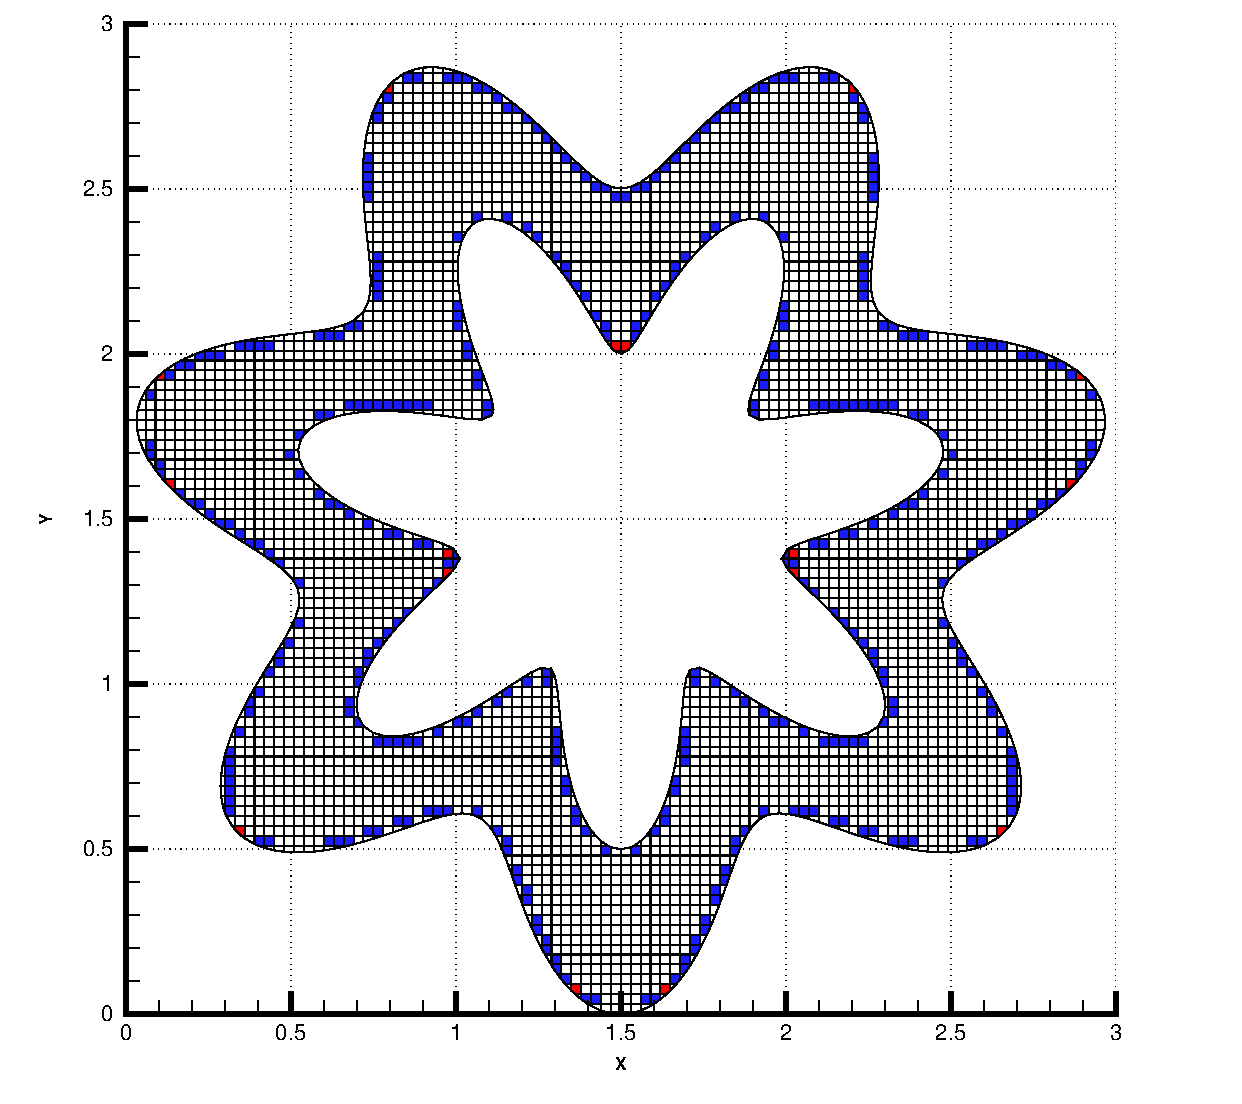
\includegraphics[width=4.5in]{figs/waveynumhoods.eps}
% \caption{\sf Domain from example XX.  Figure shows how many
% neighborhoods each cell belongs to: 
% one (white), two (blue), or three (red).
% The full example is shown in section \ref{sec:compResults}.}
% \label{fig:2nborTile}
% \end{center}
% \end{figure}

The two steps above can be part of a preprocessing step, since they do not
depend on the computed solution. For moving geometry however they would
be done at each step.
Using the merging tiles and the cell counts, the state redistribution
algorithm after one forward Euler time step is as follows:

%\begin{enumerate}[label=Step \arabic*:,leftmargin=2\parindent]
\begin{enumerate}
\item
{\bf Compute the volume-weighted and count-weighted solution for all
merged tiles.}   

\vspace*{.1in}
The contribution of each cell is divided by the number of neighborhoods 
it is part of (i.e. its count). The notation in this section refers
to cut cell $i,j$, with solution $U_{i,j}$ and volume
$V_{i,j}$. 
The provisionally updated solution before the
stabilization algorithm is applied is $\widehat{U}_{i,j}$.
There will now be many temporary merging neighborhoods which 
we denote as $\widehat{Q}_{i,j}$. 
Let $M_{i,j}$ denote the set of cell indices in the cell $(i,j)$ merging
neighborhood.  Then
\begin{equation}
\label{tiledef}
\widehat{Q}_{i,j} =  \frac{1}{{\widehat V}_{i,j}} \, \sum_{k \in M_i} \,  
\frac{V_k}{N_k}  \,\,  \widehat{U}_k
\end{equation}
where the volume ${\widehat V}_{i,j}$ is the merging tile volume similarly weighted,
\begin{equation}
\label{voldef}
{\widehat V}_{i,j} =  \sum_{k \in M_i } \,  \frac{V_k}{N_k}  .
\end{equation}

In other words, the contributions from each cell are weighted by the
number of neighborhoods they contribute to.
In the above equations, $k$ is  a multi-index ranging over the neighbors 
of cell $i,j$ included in its merging tile.
Note that most full cells will have ${\widehat V}_{i,j} = V_{i,j}$, 
and $\widehat{Q}_{i,j}  = \widehat{U}_{i,j}$.





\item
{\bf Compute a (limited) gradient for each merging
tile.}

\vspace*{.1in}
For cut cells, a least squares procedure  similar to the one used for
the finite volume update is an obvious choice. However instead of using the
solution $U_{i,j}$ on the Cartesian mesh at time $t_n$,
the merging neighborhood solution  $\widehat{Q}_{i,j}$ is used. It is important
to note that the centroid of the merging neighborhood is \textit{not} the centroid of cell ${i,j}$ (figure \ref{fig:centroids}).
\begin{figure}
    \centering
    \subfloat[]{\includegraphics[width=0.45\linewidth]{figs/centroids3.pdf}} \hfill
    \subfloat[]{\includegraphics[width=0.45\linewidth]{figs/centroids4.pdf}}
    \caption{The centroids of the Cartesian and cut cells are indicated with a solid circle ($\bullet$).  The centroids and weighted centroids of the merging neighborhoods are indicated with a square ($\blacksquare$) and a cross ($\times$), respectively. Note that the centroids and weighted centroid of the cut cell neighborhoods do not necessarily coincide.}
    \label{fig:centroids}
\end{figure}
The reconstruction neighborhood for $i,j$ is initialized to the $3 \times 3$ tile centered on $i,j$.
With this choice, it could happen that the centroids are too close to each other to compute a gradient in the normal direction (figure \ref{fig:tooclose}). If the weighted centroids are not at least $0.5\,\Delta x$  and $0.5\,\Delta y$ apart in the $x$ or $y$ direction then we increase the stencil size for the gradient computation.  For example, if the weighted centroids are too close in the $x$ direction, but not the $y$ direction, then the $5\times 3$ tile is used as the reconstruction neighborhood.  Similarly, if the weighted centroids are too close in the $y$ direction, but not the $x$ direction, then the $3\times 5$ tile is used as the reconstruction neighborhood.  The neighborhood size is increased until the distance constraint is satisfied in both directions.  In figure \ref{fig:tooclose}, the appropriate reconstruction neighborhood is $3\times 5$ reconstruction tile.
% The same neighborhood that is used for computing the gradient can be used to limit the gradient to prevent overshoots. The centroid is computed using the same weighting by number of neighborhoods as when the volume was computed. (IS THIS TRUE AND IS IT NECESSARY) NEED DISCUSSION OF NOT A REAL CENTROID
% For most full cells with a count of one, the normal gradient computation as done in the finite volume update will suffice.

\begin{figure}
    \centering
    \subfloat[]{\includegraphics[width=0.45\linewidth]{figs/tooclose2.pdf}} \hfill
    \subfloat[]{\includegraphics[width=0.45\linewidth]{figs/tooclose1.pdf}} 
    \caption{The blue cell's $3\times3$ reconstruction tile highlighted in green.  The weighted centroids are indicated with a cross ($\times$).}
    \label{fig:tooclose}
\end{figure}

\item
{\bf Replace the provisionally computed cut cell values and their adjacent
full cell neighbors with  the contributions from the merged tiles.} 

\vspace*{.1in}
The final solution at time $t^{n+1}$ on cut cell $i,j$ is obtained by compiling a the indices of all merging neighborhoods that overlap cell $i,j$ in the set $W_{i,j}$.  Then, the solution on merging neighborhood $k,l$ in $W_{i,j}$ is evaluated at $i,j$'s physical centroid, $x_{i,j}$, given by $\hat{q}_{k,l}(x_{i,j})$.  The final solution value on cell $i,j$ is given by the average of these values, i.e.,
\begin{equation} \label{eq:final_update_linear}
U^{n+1}_{i,j} := \frac{1}{N_{i,j}}\sum_{(k,l) \in W_{i,j}}\hat{q}_{k,l}(x_{i,j}).
\end{equation}
To use the example of figure \ref{fig:2nborTile}, the cut cell value
\begin{equation}
   U_{i,j}^{n+1} := \widehat{Q}_{i,j} 
   + (x_m - x_{i,j}) \, \frac{\partial \widehat{Q}_{i,j}}{\partial x} 
   + (y_m - y_{i,j}) \, \frac{\partial \widehat{Q}_{i,j}}{\partial y}
\end{equation}
since cell ${i,j}$ only belongs to one neighborhood. The adjacent full cell
on the other hand belongs to two neighborhoods -- the one it shares with
the cut cell $i,j$ , and its own merging neighborhood.
So its solution at time $t_{n+1}$  becomes
\begin{equation}
\label{eqn:numhood2ex}
\begin{split}
   U_{i,j+1}^{n+1} \,=\, & \frac{1}{2}\widehat{q}_{i,j}(x_{i,j})+ \frac{1}{2} \widehat{q}_{i,j+1}(x_{i,j}), \\
   = &\frac{1}{2} \left
   (\widehat{Q}_{i,j} 
   + (x_m - x_{i,j+1}) \, \frac{\partial \widehat{Q}_{i,j}}{\partial x} 
   + (y_m - y_{i,j+1}) \, \frac{\partial \widehat{Q}_{i,j}}{\partial y} \right ) + \frac{1}{2} \widehat{Q}_{i,j+1} .
\end{split}
\end{equation}
The last term  in eq. \eqref{eqn:numhood2ex} has no gradient terms because the
centroids of the original cell and merged cell are identical.
The fraction $\frac{1}{2}$ is because cell $(i,j+1)$ is part of  two
neighborhoods, so each contributes half of the solution.
\end{enumerate}

Different choices of neighborhoods, the minimum volume for the merging
neighborhood, gradient neighborhoods, and limiting will give
somewhat different computational results. Some of these will be examined
theoretically using model problems in one space dimension in section
\ref{sec:theory}. These choices can affect the stability limit of the
overall method.
We will also show computational results using different neighborhood
choices in section \ref{sec:compResults} in two space dimensions.

The conservation properties of the algorithm will be discussed after the
higher order SRD algorithm is presented in the next
section (PR PUT IT HERE). It will also be prseented more generally.   
OTHER THINGS HERE? DEMONSTRATE LINEARLY EXACT SECOND ORDER CONVERGENCE
HERE INSTEAD OF COMPRESULTS SECTION?

% SOMEHWERE PUT IMPLEMENTATION SUBSECTION OR AT LEAST A PARAGRAPH
% TO NOTE THAT THE CELL DOESNT KNOW WHO GIVES TO
% IT, SO THIS LOOP IS OVER GIVERS  NOT RECEIVERS.
The final update formula \eqref{eq:final_update_linear} can easily be implemented with a nested for loop in algorithm \ref{alg:finalupdate}.  
The outer loop iterates over the merging neighborhoods $i,j$ and the inner loop iterates over each cell $k,l$ in merging neighborhood $i,j$.  Each merging neighborhood $i,j$ gives a contribution $ \hat{q}_{i,j}(x_{k,l})/N_{k,l} $ to the cells $k,l$ that belong to it.
\begin{algorithm}[H]
\SetAlgoLined
$U^{n+1}(:,:) := 0$\\
 \ForAll{$i,j$}{
     \ForAll{$(k,l) \in M_{i,j}$}{
        $U^{n+1}(k,l) := U^{n+1}(k,l) + \hat{q}_{i,j}(x_{k,l})/N_{k,l} $
     }
 }
 \caption{Final solution update} \label{alg:finalupdate}
\end{algorithm}

\begin{figure}
	\subfloat[]{\includegraphics[width=0.45\textwidth]{figs/modelexample2D_1.pdf} \label{fig:2nborTile1}}
	\hfill
	\subfloat[]{\includegraphics[width=.45\textwidth]{figs/modelexample2D_2.pdf} \label{fig:2nborTile2}}
	\caption{Two-dimensional example of overlapping neighborhoods.  The unweighted centroids of cells $i,j$ and $i,j+1$ are indicated with solid squares ($\blacksquare$).} \label{fig:2nborTile}
\end{figure}


\subsection{Limiting on merging neighborhoods}
In this section we design a linearity preserving limiter for slopes on merging neighborhoods.  Designing a limiter that does not destroy the linearly preserving property is not so straightforward.  
%We demonstrate this
%In particular, we apply the LP limiter [] on slopes

\section{Computational Results}\label{compResults}

\subsection{Linear convergence study}
We solve \eqref{eq:conslaw} with the flux $\mathbf{F}(u) = [-2\pi y u, 2\pi x u]$ and initial condition
$$
u_0(x,y) = 
$$
until the final time $T = 1$ on the domain comprising two concentric discs in Figure \ref{fig:channel}.   
\subsection{Nonlinear convergence study}

\section{Conclusions}\label{sec:conc}
We have presented a  state redistribution algorithm to solve the small cell problem on cut cell meshes.  It is conservative, allows for overlapping temporary merging neighborhoods so is easy to implement, and is linearity preserving.   
Numerical experiments show that on smooth problems, second order accuracy is maintained, and the solution is not degraded by the postprocessing. For problems with shocks, the scheme maintains robustness at the cut cells.
We have shown experiments using SRD on two different base schemes, but it should be 
applicable to any underlying numerical method with
cell-centered variables.

We think that state redistribution should be applicable to 
different sets of equations, and to three-dimensional applications.
It also seems clear that the scheme can be extended to higher order accuracy, 
when used in conjunction with a 
higher order base scheme. We have already started extending this work to
3rd and 4th order accuracy. Higher order methods bring 
in many new features however, so we do not include that here.




%\subsection*{Acknowledgments} 



\bibliography{/Users/berger/references}
\bibliographystyle{plain}



\end{document}
